\documentclass[12pt]{article}

\usepackage{fullpage}
\usepackage{lmodern}

\usepackage[T1]{fontenc}
\usepackage[utf8]{inputenc}
%\usepackage[english]{babel}

\usepackage{csquotes, xpatch}
\usepackage{lineno}

\usepackage{longtable,booktabs} 
\usepackage{setspace}

\usepackage{tabto}
\usepackage{multirow}

\usepackage{enumerate}
\usepackage[shortlabels]{enumitem}

\usepackage{graphicx}
\usepackage[usenames,dvipsnames]{xcolor}
\usepackage[singlelinecheck=false]{caption}
\usepackage{epstopdf}
\usepackage{float}

\usepackage{amsmath}
\usepackage{amssymb}
\usepackage{amsthm}
\usepackage{accents}



%\usepackage[style=authoryear-ibid,backend=biber]{biblatex}
\usepackage[style=authoryear-ibid, natbib, maxcitenames=3, giveninits, backend=biber, urldate=long]{biblatex}
\addbibresource{SF_comm4.bib}

\renewcommand*{\bibinitdelim}{}
\renewcommand*{\bibinitperiod}{}
\DeclareNameAlias{sortname}{last-first}
\renewbibmacro{in:}{}
\renewcommand*{\revsdnamepunct}{}

%\DeclareFieldFormat{url}{Available at\addcolon\space\url{#1}}
\DeclareFieldFormat{url}{\url{#1}}

\renewbibmacro*{volume+number+eid}{%
  \printfield{volume}%
%  \setunit*{\adddot}% DELETED
  \setunit*{}% NEW (optional); there's also \addnbthinspace
  \printfield{number}%
  \setunit{\addcomma\space}%
  \printfield{eid}}
\DeclareFieldFormat[article]{number}{\mkbibparens{#1}}

\DeclareFieldFormat
  [article,inbook,incollection,inproceedings,patent,thesis,unpublished]
  {title}{#1\isdot}

\renewcommand*{\bibpagespunct}{\addcolon\space}  
\DeclareFieldFormat[article]{pages}{#1}

\DeclareFieldFormat{urldate}{% Reformats urldate field to read "accessed", replacing "(visted on)"
        (accessed %
        \thefield{urlday}\addspace
        \mkbibmonth{\thefield{urlmonth}}\addspace%
        \thefield{urlyear}\isdot)}



\newcommand{\e}{\mathrm{e}}		

\newcommand{\twochoices}[2]{\left\{ \begin{array}{lcc}
		\displaystyle #1 \\ \vspace{-10pt} \\
		\displaystyle #2 \end{array} \right. } 

\newcommand{\twovec}[2]{\left(\begin{array}{c} #1 \\ #2 \end{array}\right)}

\newcommand{\twomatrix}[4]{\left(\begin{array}{cc} #1 & #2 \\ 
		#3 & #4 \end{array}\right)}
		
		
		%%%%%%%%%%%%%%
		%%%%%%%%%%%%%%


\title{\Large Superfund Cleanup Time and Community Characteristics: \\
A Survival Analysis} 

\author{\normalsize Leili Solatyavari\footnote{Email: solatleili@gmail.com} \\
\normalsize Ingram Micro \\ 
\\
\normalsize Anna A. Klis\footnote{Corresponding author. Address: Zulauf Hall 510, DeKalb, IL 60115. Email: aklis@niu.edu.} \\
\normalsize Department of Economics, Northern Illinois University \\
}

\date{ } 

\begin{document}

\maketitle

\onehalfspacing

\vspace{-20pt}
\begin{abstract}
This paper investigates the correlation of socioeconomic characteristics of communities close to Superfund sites with the duration of cleanup using spatial survival analysis. Census-tract-level data is used to achieve a more accurate representation of affected areas. Overall, we find no evidence of slower cleanup in areas with higher minority population; rather, the median income of households is correlated with longer cleanup time. Additionally, sites located in communities with higher levels of education and voter turnout experience faster cleanup.

\noindent {\bf Keywords:} ArcGIS, hazardous waste, income, minority, Superfund, survival analysis, voter participation

\end{abstract}

\section*{Acknowledgments}

{We gratefully acknowledge comments from seminar participants at Northern Illinois University, participants of the 2017 meetings of the Midwest Economics Association, Chris Timmins, Lala Ma, Jay Shimshack, Matthew McGinty, Richard ``Max'' Melstrom, Jeremy Groves, and prior anonymous reviewers.}

%\section*{Transparency of Data}

%Data sources are described in Section \ref{data} of the article and were constructed by Dr. Solatyavari at Northern Illinois University through available file downloads and extraction from a Superfund site's Record of Decision. %Replication materials will be made available at Huskie Commons at \underline{https://commons.lib.niu.edu/}.

\newpage

\linenumbers
\section{Introduction}\label{intro}

Commercial and industrial waste has created thousands of hazardous sites throughout the United States over the past century \parencite{EPA2011}. From the 1940s until 1995, the Hooker Electrochemical Company disposed 21,000 tons of toxic byproducts into the Love Canal in Niagara Falls, NY. Nearby homeowners found chemicals leaking onto their lands, and health studies warned of serious diseases and possible genetic problems. In 1978, about 950 families were evacuated from their homes, and 237 homes were bulldozed \parencite{Brown1979, NRDAR2016}. This tragedy directed governmental attention, like that of Congress and the Environmental Protection Agency (EPA), to toxic lands, leading to the creation of Superfund cleanup program in 1980 under the Comprehensive Environmental Response, Compensation, and Liability Act.  In 1981, the Love Canal was the first site listed in the history of Superfund, reaching ``construction complete'' in 2004 \parencite{USEPA2018}. Superfund is the name of the environmental program and also the trust fund established to address abandoned hazardous waste sites when no responsible party is identified. %The program also provides ``a clearly defined responsibility for the polluters'' which \textcite{perrings_2000} suggests as a model for global cleanup; thus, understanding the impact of community characteristics such as income, education, and minority status on the workings of Superfund cleanup can  inform development work and similar initiatives within and beyond the US. 

The process of finding and negotiating with polluters often delays the actual start of cleanup construction, which can then vary in length depending on site pollution, chosen cleanup method, and administrative delay. This timeline concerns the public directly: in 2017 approximately 53 million people, or roughly 16\% of the US population at the time, lived within three miles of a Superfund site; of those, 15 million lived within one mile of a Superfund site, of which 44\% belong to a minority \parencite{EPA2017}. Much of the environmental justice literature considers how minority communities may bear a disproportionate burden of the risks associated with living near hazardous waste sites. \textcite{lavelle1992unequal} and \textcite{bullard2008dumping} argue that, in more than half of the ten EPA regions, the EPA chooses less desirable cleanup treatments and tends to face delays for contaminated lands in areas with a greater minority population, though \textcite{Gupta1996} find no impact of minority status on the cost-permanence trade-off of cleanup choices. 

We perform a spatial analysis using census-tract-level data to investigate the socioeconomic characteristics and engagement of Superfund communities and the correlation with the duration of cleanup. This is also our main contribution: survival analysis estimates hazard ratios, allowing for more meaningful interpretation of variable effects on cleanup duration. Additionally, using census-tract-level data achieves a finer and more accurate representation of affected areas, as opposed to larger aggregates like zip codes. Overall, we find no evidence of slower cleanup of sites in areas with a high fraction of Black or Hispanic population. However, we do find that the median income of households is {\it negatively} correlated with the speed of site cleanup: sites in poorer neighborhoods are cleaned faster, provided they were listed in the first place. Sites with older and more engaged communities, as represented by voter participation and education, have a faster pace of cleanup. Moreover, site difficulty measures like Hazard Ranking Score and Net Present Value  are associated with a prolonged cleanup time, as is federal site ownership. We also present evidence that Community Advisory Groups are important, but that their formation is likely endogenous to cleanup duration.

Section \ref{lit} describes the background of Superfund, the cleanup process, and environmental justice concerns. Section \ref{data} describes data used, while Section \ref{metrics} presents our estimation approach and results. Section \ref{conc} concludes. 
 
\section{Background}\label{lit}

%%%Superfund

Under the Superfund program, sites with serious hazards are placed on the National Priority List (NPL). This step formalizes the Environmental Protection Agency's (EPA) commitment to permanently remove the contamination, finding responsible parties, and resolving fault and cleanup funding with them. When cleanup construction is finished, the EPA monitors NPL sites for some time after to assure that all threats have been addressed. The site is then deleted from the NPL. According to the Comprehensive Environmental Response, Compensation and Liability Information System Public Access Database, at the time of writing there were 1,666 sites ``listed on the NPL,'' of which 1,161 were sites classified as ``construction complete'' and 378 sites ``deleted from the NPL.'' Figure \ref{fig1} depicts the number of site cleanups completed since the beginning of Superfund until 2010.

\begin{figure}[h] \centering
	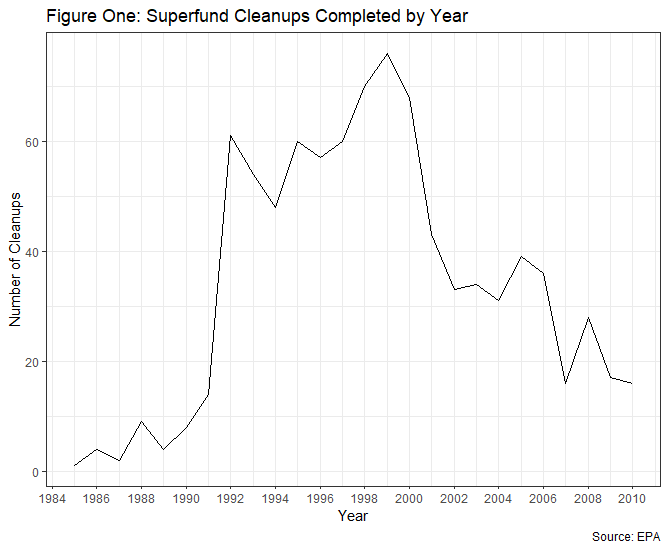
\includegraphics[width=0.75\textwidth]{fig1.png}
	\caption{Superfund cleanups completed by year.} \label{fig1}
\end{figure}

%%%Cleanup time

Cleanup time itself can vary: some communities wait a long time for cleanup completion, while other sites resolve more quickly. The length of time it takes for a site to complete the cleanup process is important to communities living nearby as they may be impacted by the contamination on the site, directly or indirectly, by the continued existence of the site. The variation in the observed cleanup duration can be divided into the two main time-frames for a Superfund site: enforcement time and actual cleanup time.

Enforcement time includes the work of identifying the responsible parties and developing a plan for the actual cleanup process while cleanup time referrers to the ''shovels in the ground'' stage when actual cleanup is occurring. Unfortunately we are unable to observe the distinct time-frames so our analysis is restricted to being a correlation analysis rather than a causation analysis. We do not; however, view this as a disadvantage given our objective of identifying which communities suffer higher costs from contamination and the fact that a longer overall duration, irrespective of time-frame, impose higher costs on the nearby residents and that only the finalization of the cleanup marks a turning point for the surrounding community.

\begin{table}[t] 
	%\renewcommand\thetable{3.1}
	\centering	 \footnotesize
	\caption{\small Summary Statistics for Superfund Sites and Population within 1 Mile of Site} \label{summstat}
	\tabcolsep 9pt
    \begin{tabular}{l|l|cccc}
    \hline
        Variable (N = 1398) & Description & Mean & Std. Dev. & Minimum & Maximum \\ \hline
        event & Completed Cleanup & 0.6819 & 0.4659 & 0.0000 & 1.0000 \\ 
        duration & Duration of Cleanup (days) & 5389.0000 & 3039.0000 & 111.0000 & 12540.0000 \\ 
        npv & NPV (\$100,000) & 143.9000 & 599.4000 & 0.0000 & 14760.0000 \\ 
        SITE\_SCORE & Hazard Ranking Score & 43.1400 & 8.6630 & 28.5100 & 84.9100 \\ 
        federal & Federally Owned Sites & 0.1196 & 0.3246 & 0.0000 & 1.0000 \\ 
        CAG & Community Advisory Group & 0.0344 & 0.1823 & 0.0000 & 1.0000 \\ 
        pop & Population & 1061.0000 & 998.6000 & 0.2249 & 5893.0000 \\ 
        permin & Percentage Minority & 0.1501 & 0.1902 & 0.0000 & 0.9868 \\ 
        pero65 & Percentage over 65 years & 0.1117 & 0.0511 & 0.0000 & 0.3667 \\ 
        unemp & Unemployment Rate & 0.0554 & 0.0533 & 0.0015 & 0.2976 \\ 
        pernhs & Percentage with no High School Degree & 0.0675 & 0.0483 & 0.0000 & 0.3878 \\ 
        perhsd & Percentage with High School Degree or GED & 0.4392 & 0.0828 & 0.0025 & 0.8094 \\ 
        percld & Percentage with a College Degree & 0.1050 & 0.0741 & 0.0004 & 0.5498 \\ 
        perocc & Percentage of Owner-Occupied Housing & 0.2396 & 0.0740 & 0.0000 & 0.3801 \\ 
        minc & Median Income (2010 \$) & 12330.0000 & 12370.0000 & 3.3510 & 76590.0000 \\ 
        vote & Voter Participation Rate & 0.5466 & 0.0490 & 0.3970 & 0.6690 \\ 
        party & Democratic Representative & 0.5029 & 0.5002 & 0.0000 & 1.0000 \\ 
        region1 & EPA Region 1 & 0.07378 & 0.2615 & 0.0000 & 1.0000 \\ 
        region2 & EPA Region 2 & 0.1633 & 0.3698 & 0.0000 & 1.0000 \\ 
        region3 & EPA Region 3 & 0.1433 & 0.3505 & 0.0000 & 1.0000 \\ 
        region4 & EPA Region 4 & 0.1347 & 0.3415 & 0.0000 & 1.0000 \\ 
        region5 & EPA Region 5 & 0.1812 & 0.3853 & 0.0000 & 1.0000 \\ 
        region6 & EPA Region 6 & 0.06734 & 0.2507 & 0.0000 & 1.0000 \\ 
        region7 & EPA Region 7 & 0.06017 & 0.2379 & 0.0000 & 1.0000 \\ 
        region8 & EPA Region 8 & 0.0394 & 0.1946 & 0.0000 & 1.0000 \\ 
        region9 & EPA Region 9 & 0.06805 & 0.2519 & 0.0000 & 1.0000 \\ 
        region10 & EPA Region 10 & 0.06877 & 0.2531 & 0.0000 & 1.0000 \\
			\hline
	\end{tabular}
\end{table}


\begin{figure}[t] \centering
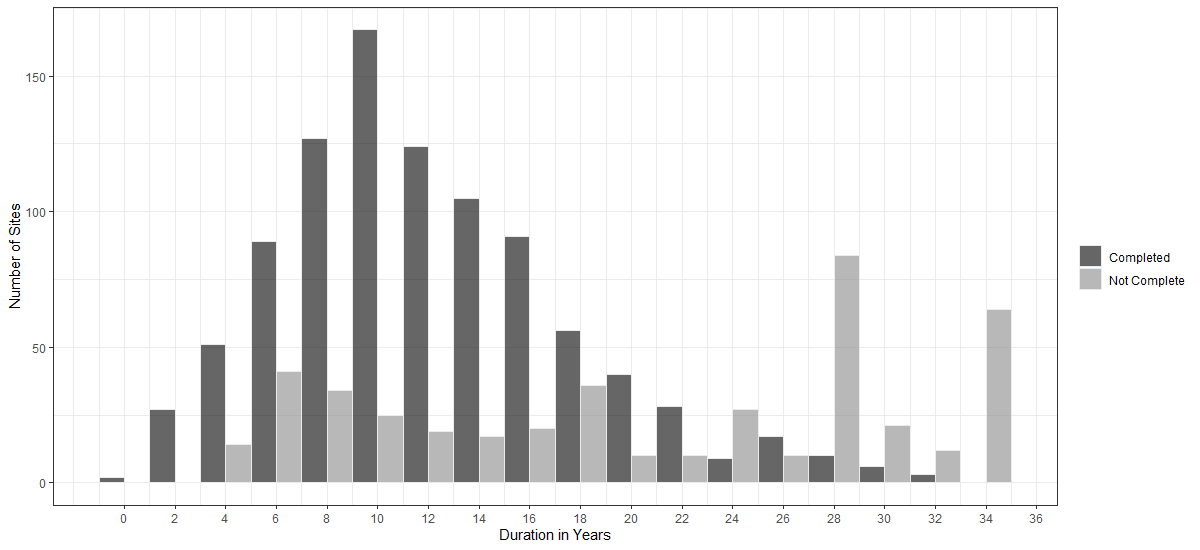
\includegraphics[width=0.75\textwidth]{fig2.png}
\caption{A combined histogram of process times for Superfund sites. The black columns show the distribution of cleanup times in 2-year bins for ``Completed'' sites. The light gray columns show the distribution of years (to February 2021) since listing date for sites listed on the NPL but which have not yet attained ``Completed'' status, including four sites that were ``Deleted from the NPL'' without having ever been ``Completed.''
\label{hist1}}
\end{figure}

For the 1,396 sites under consideration in this paper, Table \ref{summstat} lists a minimum cleanup duration of 111 days and a maximal duration of over 31 years, with a mean cleanup duration of 5,389 days ($\sim$14.8 years). Figure two shows the distribution of duration to cleanup for sites based on the quartile classification of the site score, a measure of the severity of the pollution at a given site determined by the EPA with the average site having a score of about 43.14. We in the figure that except for the lowest hazard score quartile, the more pollution at the site, the longer the cleanup duration, as one would expect. Unfortunately with the data at hand, we can can not identify the cause of the lowest category having such a wide variation of cleanup durations, specifically if it is a result of longer enforcement or cleanup times; however, these are also the sites that should impose the smallest impact on the surrounding communities.  

%%%%EJ Concerns

To gain insight into policies to increase environmental justice, it is necessary to determine the common characteristics of communities that suffer environmental costs and identify the characteristics of those same communities that can be bolstered to reduce those same costs. Our concern here is identifying the characteristics of the communities located within one mile of a Superfund site that may impact the duration of time between the site being listed on the NPL and the completion of the cleanup process. Again, while we are unable to point to a causal relationship between any identified factor and the duration of the cleanup process, we are able to identify those factors that deserve further scrutiny. Others have found that capacity expansion of commercial hazardous waste facilities is negatively correlated with voter turnout \parencite{Hamilton1995} and that Superfund sites in pro-environmental counties (measured by higher voter turnout) are more likely receive targeted, cancer-risk-eliminating cleanup \parencite{hamilton1999calculating}. \textcite{Morello-Frosch2006} observe a higher level of cancer risk due to toxic releases in areas with higher levels of ethnicity segregation. If segregated communities lack political clout over decisions on waste facility locations and pollution removal, then this results in adverse health effects for everyone in an area. 

The level of demographic data plays an important role in understanding population patterns close to these sites. Previous studies often match Superfund locations with demographic attributes through zip codes; notably, \textcite{burda2014environmental} and find evidence of racial discrimination in NPL sites prior to 1994. Newer studies of health and movement responses to pollution (e.g. the earlier-mentioned \textcite{Morello-Frosch2006}, \textcite{Gamper-Rabindran2013}, and \textcite{Depro2015}) have used census tracts. Census tracts are small, relatively permanent statistical subdivisions of a county or equivalent entity that are updated by local participants prior to each decennial census as part of the Census Bureau's Participant Statistical Areas Program. Analysis based on tract level data is expected to achieve a more accurate representation of affected areas due to increased granularity \parencite{ProximityOne2019} and a richer set of demographic data.

%({As an example of granularity, the zip code of Northern Illinois University contains eight census tracts and overlaps with five others.})

Additionally, census tracts provide more statistical uniformity between tracts, averaging a population of about 4,000, while the population of a single zip code can exceed 100,000. 

%Therefore, the analysis is expected to obtain more precise results using the more well-defined census tracts as geographic areas of interest rather than zip codes. 

%As an example, let us consider the Lake Calumet Cluster Superfund site in Chicago, IL. %Figure \ref{calumet} shows the site's location and some key information from the EPA's ``Superfund Sites Where You Live'' interactive map. 
 
%The top panel of Figure \ref{zip} shows zip code 60633, which contains the Lake Calumet Cluster, while the bottom panel shows a portion of Cook County's 2010 census tracts, with the Lake Calumet Cluster highlighted as a green dot in census tract 8388. We see that zip code 60633 is somewhat larger than census tract 8388 and, in this particular case, less centered on Superfund site.

\textcite{Aydin2006} examine population changes in census tracts around Superfund sites in Harris County, TX. Using 2.5- and 5-mile radii and multiple census years, they find that site listing comes {\it before} increases in minority population, concluding -- in contrast to \textcite{burda2014environmental} -- that environmental racism was unlikely to be the cause of Superfund site listing. However, they do find that lower income levels and higher percentages of Blue Collar workers were present near the sites prior to their listing. Though their paper examines site placement and ours examines cleanup time, the results are complementary; using census-tract-level data highlights the importance of wealth in polluted areas. In this case we will look at the census tracts within one mile of a superfund site and include demographic variables to capture race, income, and other socioeconomic factors.

The largest means of promoting environmental justice is the participation of the surrounding community in the Superfund cleanup process. The Superfund Amendments and Reauthorization Act (SARA) of 1986 ``encouraged greater citizen participation in how sites are cleaned up'' \parencite{OLEM}. The EPA informs communities at each stage of the process,  gathering input opinions about cleanup strategies. \textcite{Sigman2001} shows that community involvement in the form of voter turnout is indeed an important factor that affects the EPA's bureaucratic priorities in listing hazardous sites, while \textcite{Viscusi1999} demonstrates that regulators apply more effective cleanup actions in areas with more concerned and involved citizens. Communities have several incentives for involvement: addressing contaminated sites can mitigate serious health risks associated with pollution or prevent a decline in property values \parencite{kohlhase1991impact}. Table \ref{summstat} shows that the average voter participation rate within one mile of a Superfund site is about 55 percent and ranges from around 40 percent to as high as 67 percent.

To create a more concrete opportunity for public engagement, congress also established Community Advisory Groups (CAG) as part of the SARA legislation. These CAGs seek active community representatives to help enhancing public interest and participation in the entire cleanup process. While CAGs may be suitable for some Superfund sites, they may not be applicable to all as \textcite{daley2004policy} finds that the presence of a CAG may impose an additional cost on the EPA and lengthen cleanup time. To measure the potential impact of CAG, we include an identifier variable if a given site has an associated CAG. For our data we see that only about 4 percent of the sites have an associated CAG and that most of these sites are in the top two quartiles of pollution hazard score. 

Previous research also shows that community involvement in environmental programs can be driven by factors such education, income, and political power \parencite{daniels2012public, OEJ2017}; factors which in turn may be influenced by race and historical racial issues within the United States. In addition, the \textcite{united2003not} argues that disadvantaged communities may experience difficulty with EPA community involvement training and thus lack access to the technical data and other information necessary for environmental activism. Furthermore, newer enforcement period options such as the Alternative Dispute Resolution (ADR) program require communities to possess a certain level of education and organization in order to understand technical documents and procedures. Language and cultural differences, education and income disparities, and even a lack of trust between community members and regulatory agencies can lead to decreased engagement in community involvement programs, and thus decreased influence \parencite{EPA2011}.

Education, in particular, contributes to higher participation in politics and environmental programs, offering citizens the skills required to effectively express their concerns to politicians and regulatory organizations \parencite{verba1995voice} and to understand how bureaucratic processes function \parencite{Howell1992, rosenstone1993mobilization}. Activism depends on citizen's beliefs about the benefits, costs, and impacts of collective action \parencite{finkel1989personal}, and so communities with lower educational attainment are less likely to participate. For example, Superfund cases are 1.9 times less likely to be resolved through ADR in communities with a higher percentage of less educated residents \parencite{Collins2008}. Table \ref{summstat} shows that an average of 10 percent of the population within census tracts located within one mile of the Superfund site have at least a college degree while another 44 percent have at least a high school diploma. While the average percentage with no high school diploma is only about 7 percent, it does range as high as 38 percent in some site areas. 

Level of involvement may have less to do with individual characteristics themselves and more to do with larger socioeconomic conditions such as the impact of poverty on time evaluation \parencite{dunlap1978new, Sigman2001}: poorer individuals are more likely to spend time meeting basic economic needs, as opposed to taking active voice in environmental programs. This idea, along with the idea that individuals in poverty still suffer positive costs from sites, is shown by \textcite{nakada_2017} via theoretical model indicating low-income residents vote for higher environmental taxes because they live closer to polluted sites while if the environmental campaign requires a greater commitment than a simple vote, affluent residents have more time and resources to contribute; on a national or global level this pattern is often described as the Environmental Kuznets Curve. Furthermore, the EPA may respond to interest groups in prioritizing its resources; high-income communities can lobby for more costly, comprehensive remedies \parencite{Sigman2001, Gamper-Rabindran2013, burda2014environmental}, while {Burda et al. (2013) suggest that sites in areas with a higher fraction of population over 65 are cleaned faster, since retirees have more free time to engage in environmental programs.} The areas nearby the sites in our study show an average median income of about \$30,000 ranging from as low as \$275.00 to as high as \$113,600. 

High income individuals may also face a higher cost from nearby wastelands -- especially those proposed and listed as Superfund sites -- due to depressed property values \parencite{McClelland1990}. \textcite{ready2010landfills} shows that residential property values decrease by 12.9\% on average if a landfill is located nearby; this loss can extend three or more miles from a site and can lead to urban decay or ``reverse gentrification,'' where affluent whites move away, while poor and/or minority groups take advantage of affordable housing and move in. Fixing undesirable sites, however, leads to an improvement in housing prices \parencite{Haninger2017}. In the one-mile areas around the sties in our study, about one-quarter of the homes are owner-occupied.

\section{Data}\label{data}

%In this section, we describe the data used in our investigation of community involvement's effect on the enforcement and cleanup process of Superfund sites. We use survival analysis to estimate factors that influence the time from the listing date on the National Priority List (NPL) to completion of cleanup for sites in the sample. 

Our data is derived from four sources on Superfund sites. Data on dates of Superfund lifetime events and site characteristics are collected from the Environmental Protection Agency (EPA). Information regarding latitude and longitude of Superfund sites are extracted from NASA's Socioeconomic Data and Applications Center, managed by Colombia University. Demographic data by census tracts, as well as Geographic Information System (GIS) boundary files, come from the National Historical Geographic Information System (NHGIS), provided by the Minnesota Population Center at the University of Minnesota. The NHGIS survey contains a very broad set of demographic variables from the 1980, 1990, 2000 and 2010 Decennial Censuses. Finally, voter turnout and Congressional Representative party are extracted from the US Census Bureau historical voting database. 

The research sample consists of 1,666 Superfund sites across the United States, which are either currently on the National Priority List (NPL) or deleted from the NPL. Since the US was not completely covered in census tracts in 1980, several sites are dropped due to lack of data, leading to 1,396 sites for use in cross-sectional analysis. Each of the Superfund sites are then mapped, using their latitude and longitude and ArcGIS intersects the US Census Tract boundary files with one-mile buffers around each of the centroids of the Superfund sites. Since the buffers are not fully contained within census tracts, we create a weighted sum of the characteristic data based on the share of the specific census tracts is located within the buffer and the share of the total buffer area that is made up that portion of that specific census tract. More specifically, for each census characteristic, the value used in this analysis is calculated as shown below:

\begin{equation}
X(t)=\displaystyle\sum_{n=1} ^{j} \Big[\frac{\text {area of buffer-track intersection}}{\text {area of census tract}}\times x_j] \times \frac{\text {area of buffer-track intersection}{\text area of buffer}}  \label{wght_cen}
\end{equation}

The main trade-off between tract-level and zip-code-level data is census collection timing. This paper relies on the full US population demographics captured in the main Decennial Census \parencite{USCensus}. Specifically, we use the 1980 census to capture the demographics for sites listed between 1980 to 1989, and similarly for other decades. In this way, factors that influence the cleanup process are pre-determined with respect to the cleanup duration. One concern with using this data is potential endogeneity being caused by changing demographics between the start and ending of the cleanup. {\textcite{Depro2015} mention issues with census-tract data when investigating migration; the decennial data entries do not adequately capture demographic changes caused by those ``fleeing from'' and ``coming to the nuisance.'' First, the structure of survival analysis makes this a non-issue is that it is assumed that the non-treatment control variables remain fixed over the lifetime of the analysis. Secondly, as stated previously, we are not attempting to determine causality, only correlation to identify the potential areas of concern or success in a move toward increasing environmental justice in EPA cleanups. We also include a robustness check with centered listing, meaning that sites listed between 1985 and 1995 are linked with data from the 1990 Census, to test for the sensitivity of our analysis to the linking of census data. 

%This is also why we use cross-sectional analysis instead of a panel approach.

Demographic variables of interest include the fraction of population that are classified as minority defined as non-white population, the unemployment rate, levels of education via the percentage of those with high school diplomas and those with a college degree (using the percentage with no high school degree as the reference group), the median household income measured as the inverse hyperbolic sine of the median income,\footnote{The inverse hyperbolic sine transformation is similar to the log transformation but avoids the problems caused by observations with zeros or ones} the percentage of homes that are owner occupied, and the percentage over 65 years. 

Table \ref{summstat} presents the summary statistics for the relevant community characteristics and control variables near Superfund sites. Cleanup completion occurs for 68\% of sites in our dataset, and the average time of cleanup is 5,389 days ($\sim$14.8 years). With regard to different time periods, cleanup is finished for 83\% of sites listed during the 1980s (with 5,858 days average duration), 65\%  listed in the 1990s (5,385 days), 20\% from the 2000s (4,218 days), and for only 1\% of sites listed during the 2010s (2,192 days). The sample consists of 1,229 non-federal sites and 167 federal sites, while the average present worth of a site's cost is \$14,390,000. The average population within a one-mile radius of a Superfund site is 1061 people earning a median yearly income of \$12,330.\footnote{We scale the median income using the inverse hyperbolic sine transformation which is similar to the natural log yet avoids the problems with values approaching zero.} The average buffer area has an average minority population of about 15\% ranging from as low as zero to as high as 98\%.  

%In some of our specifications, the fraction minority variable is broken down into four segments and controlled as a categorical variable. The categorical variable shows that 54\% of sites have a ``true'' minority population of less than 25\% Black or Hispanic within one mile of a Superfund site, while 19\% of Superfund sites are located in areas with a high rate of minority population estimated between 76 and 100\%.  

Since measures of direct public participation in Superfund site cleanup do not exist, we use voter turnout and the existence of a Community Advisory Group (CAG) near the site as proxies for the level of public participation. Voter turnouts for presidential elections 1980-2012 are matched based on the state where the Superfund is located and the closest presidential election date to the site's listing date. Unfortunately, we do not have detailed data on the formation timelines of CAGs, which are formed in response to site listing or duration, nor on the existence of any unofficial community organization efforts. We see an average of about 55\% voter participation ranging from near zero to as high as 67\%. 

We do include site-specific characteristics, including the total present value of site remediation cost (NPV). Cost information for each site is available in its Record of Decision (ROD), available on the EPA website. Each ROD summarizes the details of the planned cleanup implementation, breaking down the estimated total present value into capital costs, which represent the actual cleanup construction costs, as well operation/maintenance costs, which comprise the annual costs of the selected remedy's administration and up-keep. Each ROD also presents detailed information regarding which costs are discounted and the discount rate used. Much of the sample used a 7\% discount factor, in accordance with policy from the former Office of Solid Waste and Emergency Response (OSWER), now the Office of Land and Emergency Management.\footnote{The importance of discount factors is described in the 2000 ``Guide to Developing and Documenting Cost Estimates During the Feasibility Study'' from the EPA and US Army Corps of Engineers, and OSWER's 7\% default is mentioned throughout 1999's ``Guide to Preparing Superfund Proposed Plans, Records of Decision, and Other Remedy Selection Decision Documents.''} The present value is thus an estimate of the entire expected cost of the remediation. We reviewed site RODs and manually extracted the stated net present worth of cleanup cost of the site's chosen method for the sample {To keep NPVs consistent, we recalibrated any sites that did not use the 7\% discount factor.} As with the median income, we also transform this variable using the inverse hyperbolic sine transformation.

The nature of site contamination can also dictate the length of cleaning time.\footnote{Contaminated media usually include debris, groundwater, sediment, surface water, or waste, and the type of contaminants are acids, metals, Volatile Organic Compounds and Polycyclic Aromatic Hydrocarbons substances. Generally, cleanup is easier if the contaminated media is waste or debris, while it is much harder for groundwater or soil.} \textcite{Gupta1996} find that the EPA prefers permanent cleanup techniques, but not at any cost. To account for the nature of the pollution, we use the Hazard Ranking Score (HRS) scaling from 0 to 100, calculated by the EPA to show the level of toxicity and cleanup difficulty in sites. Sites with a higher HRS possess higher levels of contaminants and the average site in our sample has a score of 43.14 ranging from as low as 28.51 to has high as 84.19. Naturally, we expect that the more polluted a site, the longer cleanup construction will take. Apart from technical difficulties caused by contamination level, organizational behavior may further hinder the process of cleanup: \textcite{daley2004policy} find evidence that the EPA pays less attention to highly-contaminated sites and more to low-risk sites. Administrative convenience may decrease the likelihood of quick and full cleanup as the level of site difficulty increases; the organization is able to tackle a larger number of cleanup tasks if it prioritizes ``easy sites'' and shifts efforts away from ``difficult sites.'' In our analysis we utilized both the direct score and categorical variables dividing the sites into quartiles based on the scores as demonstrated in Figure 2.

Site ownership might also contribute to cleanup time. Since cleanup time is defined as the length of time between listing and reaching ``construction complete'' status, any delays in identifying and possibly litigating Potentially Responsible Parties (PRPs) are captured in total cleanup time. Certain sites belong to federal facilities (i.e. military branches, Department of Defense, Department of Energy), so we include an indicator for whether the Superfund site belongs to a federal facility. Without a full organizational investigation, it is difficult to say whether government ownership would shorten or lengthen cleanup time. In such a case, the regulator (EPA) and the regulated (federal site owners) belong to the same entity, the US government, which does not sue itself except under rare occasions of constitutional crisis. Therefore, it is possible that government ownership could avoid lengthy court battles and thus shorten cleanup time. However, since the funding source for the project must ultimately come from taxpayers, the EPA may lack incentive to establish quick funding responsibility from an outside party, while the federal offices involved may take additional time to negotiate the handling of cleanup and its payment or may even need to wait for additional funding from the legislative branch. 

We also control for the availability of resources to accommodate fast and efficient enforcement and cleanup process with regional indicators. Figure \ref{map} maps which EPA regions serve which states; certain EPA Regions also serve tribal nations. Resources and funding allocation may vary across EPA-designated regions. State spending derives from site frequency, whether PRPs perform the cleanup, and population density. From 1999-2013, the EPA spent the most Trust Fund dollars on site cleanup in Region 2. This region includes New York and New Jersey and has a considerable number of large sites with no responsible parties found. The EPA spent about \$2.5 billion in this region, comprising about 32\% of the total cleanup funds on non-federal NPL sites during that time \parencite{GAO2015}. The methods of assigning pollution responsibility and recouping funding also vary across Superfund regions: \textcite{church2001cleaning} find that Regions 3 and 10 utilize alternative dispute resolution more often, while Regions 2 and 5 tend to litigate. Thus, we include dummies to control for unobserved differences at the regional level.
 
 \begin{figure}[H] \centering
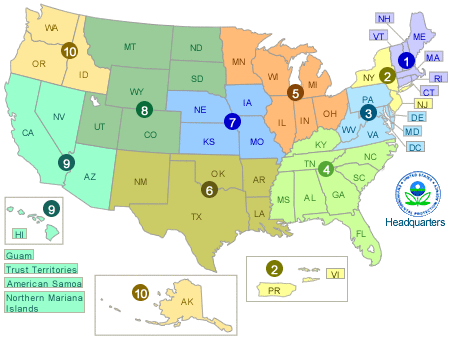
\includegraphics[width=0.75\textwidth]{us-regions.png}
\caption{\small A map from the EPA's website showing the ten EPA regions (\underline{https://www.epa.gov/aboutepa/visiting-regional-office}). \label{map}}
\end{figure}

Finally, questions of environmental protection are rather politicized in the United States. To control for any unobserved heterogeneity caused by local party preference, we include a binary variable equal to one if the district hosting the Superfund site is Democratic-controlled and zero if the district is Republican-controlled. To add this variable to the analysis, a district layer for the 97$^\mathrm{th}$ and 114$^\mathrm{th}$ Congressional assemblies is intersected with previous layers (demographics and CAG) in ArcGIS.

\section{Empirical Models and Findings}\label{metrics}

We use survival analysis to estimate the length of time from final listing on the National Priority List (NPL) until cleanup completion and how this time relates to various demographic characteristics of the affected community and site-specific characteristics.  
\newcommand{\comm}{\mathrm{CommunityChars}_i}
%Survival analysis can demonstrate how the demographic and site-specific characteristics of a Superfund site are correlated with the length of time in the cleanup process. 

Survival analysis applies when subjects are tracked until an event occurs (called ``failure'' in the jargon; success of cleanup completion is a failure of survival). In our study, the ``event'' has happened for sites which have reached ``construction completion'' status. The sites which have not reached this point are right-censored as we cannot observe their full survival time. Additionally, we are interested in the {\it risk} of failure, called the hazard ratio, which can only be measured by this econometric method; in our analysis, the hazard ratio represents the likelihood of site reaching the cleanup construction status. 

The survival function $S(t)$, denotes the probability of duration from the starting point of study until time $t$: 

\begin{equation}
S(t)=\operatorname{Prob}(T_i>t)=1-F(t)  \label{surv}
\end{equation}
where $T_i$ denotes the time until which Superfund site $i$ is still ``alive'' or not yet cleaned, and $F(\cdot)$ is the cumulative distribution function of survival times. Thus $F(t)$ measures the probability of survival -- remaining on the NPL -- until time $t$.

We estimate the length of time from listing date to cleanup completion date with Cox proportional hazards regression analysis, a semi-parametric method which allows us to determine how different variables affect the hazard. 
Using an exponential distribution, the model takes the form:

\begin{equation}
\lambda_{i}(t|X_{i}) =\lambda_{0}(t)\exp(\beta \comm + \gamma X_{i}) \label{PH1}
\end{equation}

where both $\comm$ and controls $X_{i}=(x_{i1}, x_{i2},..., x_{ik})$ are column vectors of covariates for site $i$, $\beta$ and $\gamma$ are row vectors of regression coefficients, $\lambda_{i}$ is the expected hazard calculated for each subject at the time that construction completion takes place, and the baseline hazard $\lambda_{0}$ represents the probability of event occurrence when all explanatory variables have zero value. The interpretation of the hazard ratio (H.R.) is more straightforward. As an illustration, if we consider two sites, $i = \{1, 2\}$, with covariates $X_{1}$ and $X_{2}$, then the ratio of their hazards at time $t$ is:

\begin{equation}
\frac{\lambda(t|X_{1})}{\lambda(t|X_{2})}=\frac{\lambda_{0}(t) \exp(\gamma X_{1})}{\lambda_{0}(t) \exp(\gamma X_{2})}=\frac{\exp(\gamma X_{1})}{\exp(\gamma X_{2})}=\exp(\gamma(X_{1}-X_{2}))
\end{equation}

Thus the hazard ratio depends on the difference between two sites' covariates. If there is only one covariate considered ($k=1$), and if the difference in the two sites' explanatory variable is exactly one unit ($x_{11}- x_{21}=1$), then the hazard ratio is the exponential of the regression coefficient (H.R. $= \e^{\gamma_1}$). A hazard ratio greater than one indicates that a unit increase in the variable of interest increases the ``hazard'' and thus \emph{decreases} the duration of cleanup completion, whereas a hazard ratio of less than one indicates less hazard, a higher likelihood of survival, and thus \emph{lengthens} the cleanup duration. For interpretation, if a hazard ratio is greater than one, a unit increase in the variable increases the probability of event occurrence by a percentage of $(\mathrm{H.R.}-1)\times100$. 

One concern with this analysis is that both technology and other factors that are not observed may change across the decades causing the timing of any combination of the enforcement and cleanup periods to change. To address this concern, we assume that the sites in our sample display frailty within the survival framework. When estimating a survival model assuming frailty one is assuming that there are unobserved factors that impact all observations within a particular group in the same way, but may impact groups differently. The most logical example is assuming that all men and all women are impacted by some unobserved factor in the same way within their gender, but the impact on men and women differ across genders. In the framework of this analysis we define our grouping as the start year for each of the sites and assume frailty across those start years. Therefore we are allowing unobserved factors to impact all sites that start in a particular year the same way; however, we assume that those unobserved factors impact sites that start in different years differently.

To implement this methodology in the Cox Proportional Hazard model framework, we will estimate a mixed-effects model using the coxme package available in R. This method adds a random effect to equation \ref{PH1} such that it becomes

\begin{equation}
\lambda_{i}(t|X_{i}) =\lambda_{0}(t)\exp(\beta \comm + \gamma X_{i} + \delta Z_{j}) \label{PH1}
\end{equation}

where the $Z_{j}$ denotes the group over which frailty is assumed, in our case the start year, and $\delta$ can be considered a shift factor which will shift the baseline hazard function to account for the unobserved factors impacting projects started in year $j$. When implemented, the coxme package reports the variance and standard deviation of the estimated $\delta\ coefficients to give an idea as to the distribution of frailty effects. 

Table \ref{cox1} presents the first specifications of the Cox proportional hazards model with and without the frailty assumption analyzing Superfund cleanup time. Columns 1 and 2 includes only the socioeconomic characteristics of census tracts within one mile of Superfund sites, columns 3 and 4 include two measures of community participation and two measure of site quality, and columns 5 and 6 replace the continuous measure of the site hazard score with the quintiles.  

\begin{table}[t]
    \centering	\footnotesize
	\caption{\small Cox regression estimates of cleanup time within one mile of a Superfund site with and without frailty assumed across site Start Year, basic specification including socio-economic, participation, and some site characteristics only.} \label{cox1}
	\tabcolsep 9pt
		\begin{tabular}{l|cccccc}
    \hline
        Variable & (1) & (2) & (3) & (4) & (5) & (6) \\ \hline
        permin & -0.472** & -0.425* & -0.229 & -0.223 & -0.450** & -0.529** \\ 
        ~ & 0.214 & 0.221 & 0.222 & 0.228 & 0.224 & 0.23 \\ 
        pero65 & 0.605 & 0.868 & 0.597 & 0.838 & 1.101 & 1.345* \\ 
        ~ & 0.814 & 0.815 & 0.808 & 0.813 & 0.787 & 0.792 \\ 
        unemp & 1.631** & 1.133 & 1.595** & 1.317* & 1.085 & 0.934 \\ 
        ~ & 0.687 & 0.711 & 0.688 & 0.701 & 0.715 & 0.722 \\ 
        perhsd & -1.123** & -1.879*** & -1.049** & -1.732*** & -0.545 & -1.511** \\ 
        ~ & 0.506 & 0.579 & 0.511 & 0.572 & 0.539 & 0.591 \\ 
        percld & -1.615*** & -1.836*** & -1.436** & -1.72*** & -0.614 & -1.215** \\ 
        ~ & 0.548 & 0.599 & 0.561 & 0.6 & 0.567 & 0.601 \\ 
        lnminc2 & -0.008 & 0.007 & -0.004 & 0.006 & -0.022 & -0.009 \\ 
        ~ & 0.026 & 0.027 & 0.027 & 0.027 & 0.027 & 0.028 \\ 
        perocc & 2.628*** & 3.187*** & 2.860*** & 3.207*** & 1.529** & 2.066*** \\ 
        ~ & 0.658 & 0.689 & 0.657 & 0.682 & 0.667 & 0.687 \\ \hline
        vote & ~ & ~ & 1.969*** & 2.184*** & 2.081*** & 2.185*** \\ 
        ~ & ~ & ~ & 0.729 & 0.737 & 0.714 & 0.718 \\ 
        CAG & ~ & ~ & -0.674*** & -0.612** & -0.835*** & -0.772*** \\ 
        ~ & ~ & ~ & 0.24 & 0.242 & 0.24 & 0.242 \\ \hline
        npv2 & ~ & ~ & -0.098*** & -0.097*** & -0.081*** & -0.078*** \\ 
        ~ & ~ & ~ & 0.016 & 0.016 & 0.016 & 0.016 \\ 
        SITE\_SCORE & ~ & ~ & -0.017*** & -0.01** & ~ & ~ \\ 
        ~ & ~ & ~ & 0.004 & 0.004 & ~ & ~ \\ 
        q\_siteslow\_haz & ~ & ~ & ~ & ~ & 0.851*** & 0.899*** \\ 
        ~ & ~ & ~ & ~ & ~ & 0.083 & 0.084 \\ 
        q\_siteshg\_haz & ~ & ~ & ~ & ~ & -0.275*** & -0.19** \\ 
        ~ & ~ & ~ & ~ & ~ & 0.092 & 0.096 \\ 
        q\_sitesv\_hg\_haz & ~ & ~ & ~ & ~ & -0.287** & -0.189 \\ 
        ~ & ~ & ~ & ~ & ~ & 0.116 & 0.119 \\ \hline
        Observations & 1,396 & 1,396 & 1,396 & 1,396 & 1,396 & 1,396 \\ 
        Events & 952 & 952 & 952 & 952 & 952 & 952 \\ 
        Log Likelihood & -6229.55 & -6191.68 & -6188.59 & -6167.54 & -6097.72 & -6081.52 \\ 
        AIC & 12473.11 & 12425.20 & 12399.16 & 12377.73 & 12221.45 & 12205.32 \\ 
        Variance of Random Effects & ~ & 0.13006 & ~ & 0.06273 & ~ & 0.03566 \\ 
		\hline
		\addlinespace[1ex]
			\multicolumn{3}{l}{\textsuperscript{***}$p\leq0.01$, 
				\textsuperscript{**}$p\leq0.05$, 
				\textsuperscript{*}$p\leq0.01$}
    \end{tabular}
\end{table}

Columns 1, 3, and 5 assume no frailty while columns 2, 4, and 6 assume there is frailty shared by the start year of the Superfund site. In comparing the column pairs we see that for most cases the assumption of frailty does not impact the statistical significance of the variables and only slightly alters the magnitude of the estimates. [enter diagnostic]

Except for when the continuous site score measure is used, results show that areas with higher minority populations see slower cleanup time as indicated by the negative coefficient. When the continuous measure of the site score is used we see the sign of the percentage of minority variable remains negative indicating there is still a slower cleanup time; however, we loose statistical significance. This is likely impacted by the fact that, as observed in Figure 2, there is a non-linear impact of site score on cleanup time with sites with the lowest score seeing longer cleanup times than those with mid-range scores which, in turn, see shorter cleanup times compared to high site scores. Given this we argue that the quintile measure is a better measure as it allows for this non-linear effect and the magnitude of the percentage of minorities effect is similar to that in columns 1 and 2.

In the case of higher percentage of those over sixty-five and the measure of median income, we see no statistically significant impact except for in the final specification; however, the coefficient estimates are positive indicating that if there was a statistical impact, it would speed up cleanup. The more unemployment seen in the area, the faster the cleanup process in all of the columns; however, the effect is only significantly in columns 1, 3, and 4. The final characteristic variable that is correlated with faster cleanup times is the percentage of homes that are owner occupied. These results are very large indicating that areas with more owner-occupied homes see much faster cleanup as one would expect given the potential for both health and financial costs via lost home value caused by the Superfund sites. 

In terms of education the coefficients on both the percentage of the population with a high school degree and the percentage of the population with a college degree are both negative and statistically significant indicated a slower cleanup time compared to areas with no high school degree. At first this may seem surprising as education would seem to be an indicator of more participation in the cleanup process; however, the subsequent columns in Table \ref{cox1} indicate that this potential for increased participation may, in fact, be related to longer cleanup times. Recall that Community Advisory Groups (CAG) only exist in about three percent of our sample; however, we see very significant negative impact from the existence of these groups across specification with and without frailty. These results clearly indicate the need to be able to split the cleanup time into both the enforcement and cleanup processes to state conclusively if more activism by the community slows cleanup, but the correlation is clear. 

Voter participation is also used as a proxy for community activism in columns three through six and the show that areas with higher voter turnout also see faster cleanup. This may very well be an indication that voting may be a different form of participation in the process, namely it may be measuring political pressures being applied by incumbents to speed the process to ensure positive responses from voters in the area. Again, we would need data splitting the cleanup time between the two key components leaving this as merely a conjecture. The remaining coefficient estimates indicate that more expensive cleanup processes take longer with the negative coefficient on the adjusted NPV variable and the site score coefficients are in line with the observations from Figure 2 previous. 

\begin{table}[!ht]
	\centering	\footnotesize
	\caption{\small Cox regression estimates with frailty of cleanup time within one mile of a Superfund site with additional controls and interactions added.} \label{cox2}
	\tabcolsep 9pt
    \begin{tabular}{l|cccc}
    \hline
        Variable & (1) & (2) & (3) & (4) \\ \hline
        permin & -0.789*** & 3.817* & -0.74*** & -0.8*** \\ 
        ~ & 0.253 & 2.301 & 0.254 & 0.254 \\ 
        pero65 & 0.669 & 0.576 & 0.759 & 0.718 \\ 
        ~ & 0.794 & 0.796 & 0.795 & 0.793 \\ 
        unemp & 0.414 & 0.5 & 0.406 & 0.401 \\ 
        ~ & 0.75 & 0.755 & 0.753 & 0.753 \\ 
        perhsd & -0.93 & -0.823 & -1.172 & -0.895 \\ 
        ~ & 0.6 & 0.604 & 0.733 & 0.6 \\ 
        percld & -0.02 & 0.021 & 0.849 & -0.015 \\ 
        ~ & 0.628 & 0.63 & 0.835 & 0.628 \\ 
        lnminc2 & -0.018 & -0.018 & -0.016 & -0.017 \\ 
        ~ & 0.03 & 0.03 & 0.03 & 0.03 \\ 
        perocc & -0.322 & -0.419 & -0.299 & -0.435 \\ 
        ~ & 0.753 & 0.756 & 0.759 & 0.755 \\ \hline
        vote & 0.426 & 1.504 & 0.355 & 0.548 \\ 
        ~ & 1.107 & 1.225 & 1.109 & 1.108 \\ 
        CAG & -0.728*** & -0.724*** & 0.502 & -0.294 \\ 
        ~ & 0.246 & 0.246 & 2.006 & 0.586 \\ 
        npv2 & -0.108*** & -0.107*** & -0.107*** & -0.108*** \\ 
        ~ & 0.017 & 0.017 & 0.017 & 0.017 \\ 
        q\_siteslow\_haz & 0.837*** & 0.842*** & 0.843*** & 0.853*** \\ 
        ~ & 0.086 & 0.086 & 0.086 & 0.086 \\ 
        q\_siteshg\_haz & -0.183* & -0.18* & -0.177* & -0.174* \\ 
        ~ & 0.097 & 0.097 & 0.097 & 0.098 \\ 
        q\_sitesv\_hg\_haz & -0.144 & -0.15 & -0.15 & -0.171 \\ 
        ~ & 0.121 & 0.121 & 0.121 & 0.124 \\ \hline
        party & 0.064 & 0.059 & 0.052 & 0.059 \\ 
        ~ & 0.077 & 0.092 & 0.389 & 0.077 \\ 
        FEDERAL & 1.11*** & 1.106*** & 1.107*** & 1.123*** \\ 
        ~ & 0.144 & 0.144 & 0.144 & 0.144 \\ 
        REGION2 & 0.017 & 0.061 & -0.012 & 0.022 \\ 
        ~ & 0.156 & 0.158 & 0.157 & 0.156 \\ 
        REGION3 & 0.208 & 0.246 & 0.186 & 0.213 \\ 
        ~ & 0.155 & 0.157 & 0.156 & 0.156 \\ 
        REGION4 & 0.438** & 0.459** & 0.408** & 0.445** \\ 
        ~ & 0.184 & 0.185 & 0.185 & 0.185 \\ 
        REGION5 & 0.363** & 0.363** & 0.346** & 0.363** \\ 
        ~ & 0.147 & 0.147 & 0.148 & 0.147 \\ 
        REGION6 & 0.699*** & 0.712*** & 0.675*** & 0.707*** \\ 
        ~ & 0.203 & 0.205 & 0.203 & 0.203 \\ 
        REGION7 & 0.307 & 0.327* & 0.283 & 0.301 \\ 
        ~ & 0.194 & 0.195 & 0.195 & 0.195 \\ 
        REGION8 & 0.269 & 0.288 & 0.207 & 0.253 \\ 
        ~ & 0.235 & 0.236 & 0.238 & 0.236 \\ 
        REGION9 & -0.304 & -0.365 & -0.319 & -0.285 \\ 
        ~ & 0.235 & 0.247 & 0.236 & 0.236 \\ 
        REGION10 & 0.696*** & 0.73*** & 0.685*** & 0.709*** \\ 
        ~ & 0.177 & 0.178 & 0.177 & 0.177 \\ \hline
        permin:vote & ~ & -8.793** & ~ & ~ \\ 
        ~ & ~ & 4.423 & ~ & ~ \\ 
        permin:party & ~ & 0.017 & ~ & ~ \\ 
        ~ & ~ & 0.434 & ~ & ~ \\ \hline
        permin:CAG & ~ & ~ & -3.525 & ~ \\ 
        ~ & ~ & ~ & 2.739 & ~ \\ 
        perhsd:party & ~ & ~ & 0.353 & ~ \\ 
        ~ & ~ & ~ & 0.827 & ~ \\ 
        percld:party & ~ & ~ & -1.492 & ~ \\ 
        ~ & ~ & ~ & 1.045 & ~ \\ 
        perhsd:CAG & ~ & ~ & -1.474 & ~ \\ 
        ~ & ~ & ~ & 3.836 & ~ \\ 
        percld:CAG & ~ & ~ & -1.873 & ~ \\ 
        ~ & ~ & ~ & 3.136 & ~ \\ \hline
        CAG:q\_siteslow\_haz & ~ & ~ & ~ & -0.894 \\ 
        ~ & ~ & ~ & ~ & 0.72 \\ 
        CAG:q\_siteshg\_haz & ~ & ~ & ~ & -0.689 \\ 
        ~ & ~ & ~ & ~ & 0.831 \\ 
        CAG:q\_sitesv\_hg\_haz & ~ & ~ & ~ & 0.326 \\ 
        ~ & ~ & ~ & ~ & 0.723 \\ \hline
        Observations & 1,396 & 1,396 & 1,396 & 1,396 \\ 
        Events & 952 & 952 & 952 & 952 \\ 
        Log Likelihood & -6020.40 & -6018.52 & -6018.21 & -6017.93 \\ 
        AIC & 12110.04 & 12110.02 & 12115.60 & 12111.21 \\ 
        Variance of Random Effects & 0.06566 & 0.06437 & 0.06582 & 0.06702 \\ \hline
    	\addlinespace[1ex]
			\multicolumn{3}{l}{\textsuperscript{***}$p\leq0.01$, 
				\textsuperscript{**}$p\leq0.05$, 
				\textsuperscript{*}$p\leq0.01$}
	\end{tabular}
\end{table}

Table \ref{cox2} shows the estimates for the frailty models only when various other controls and interactions are added to the specification. The first column adds indicators for the party of the representative for the district within which the site is located, sites that are already owned by Federal government agencies and the regional variables. The party of the representative is not statistically significant in any specification nor is the effect, albeit positive, very economically significant. Sites owned by entities in the Federal government show significantly faster cleanup times, as one would expect, but we would need to be able to split the given duration into the enforcement and cleanup periods to know clearly attribute this to faster enforcement phases. 

The addition of the regional indicators (with Region 1 acting as the group reference) are interesting not necessarily for their own estimated coefficients, but the impact on other coefficients in the model. In and of themselves, only regions four, five, six and ten show statistically significant impacts and in all cases they see slightly faster cleanup times compared to the reference group. As discussed previously, this may be an indication that these regions use different processes for the cleanup process causing faster resolution. 

The most interesting impact from adding the control variables is that the magnitude on the minority, college degree, owner occupied and unemployment rates all decrease indicating that the variables where previously capturing regional effects as well. Referring back to Figure three we see that regions four and five cover the entire region of the U.S. that would be classified as ''The South``, region five captures the eastern most ''Midwest``, and region ten captures the area classified as the ''Northwest``. One can easily draw connections between generalization about these areas within the United States and the variables that most impacted by the inclusion of the regional controls.\footnote{It is also interesting to note that region nine, the only region to have a negative coefficient estimate indicating a slower cleanup time, the same region that includes California. The lack of significance could likely be tied to the fact that the region also includes Nevada and Arizona which include a great deal of Federally owned sites as well.}

The addition of the regional controls cause all of the characteristic controls to loose significance with the exception of the percentage of minorities in the area. In the case of the percentage of individuals with a college degree, coefficient moves closer to zero (less of a negative impact on duration) while the coefficient on percentage of owner-occupied homes changes sign. If this was a causal study, we would need to further dive into this change to determine if it is case of a high correlation between population in the United States and the EPA regions. 

The largest impact from the regional controls is the very large impact on the coefficient for the percentage of minorities variable which indicates that cleanups are even slower in areas with more minorities than before we controlled for region. While we can not confirm that this effect is independent of the possible correlation of regional definitions and geographic population distributions, even in that case, the results indicate there is something different about regions four, five, six, and ten that may speed up the process, but One alternative explanation for this could be that if there is a very high correlation between the regional definitions and U.S. population distributions, This seems to strengthen the case for further investigation into a causal link between minorities and cleanup times. 

Column two begin to add interaction variables by adding an interaction between the percentage minority variable and the voter participation and representative's party affiliation. The later interaction is not signficiant and is very close to zero and has no impact on the party measure itself. The interaction between vote participation and minorities; however, is significant and is very large is abosolute value indicating a very large slowing of cleanup. While the positive, large, and significant coefficient estimation on the minorities variable seems promising, it must be taken with the interaction coefficient. From the perspective of a given level of voter participation, increasing the percentages of minorities will significantly slow the cleanup period for a Superfund site. Likewise, for a given level of minority population, increasing voter participation will also slow the cleanup process. While this is a very interesting result; again caution must be taken because we are unable to determine if the cause is due to something in the enforcement period or these factors impacting something in the actual cleanup process. The latter effect does seem to indicate, as we noted previously with the CAG coefficient in both tables, increased participation does seem to indicate slower cleanup times. 

Column three replaces these interactions with interactions between the CAG indicator and the percentage of minorities (which might shed some light on the voter participation result just discussed), percentage of high school diplomas, and percentage of college degree holders. In all three cases the estimates are not statistically significant; however, all three show negative signs indicating slower cleanup in the presence of CAGs The lack of CAG observations is likely the cause of the addition of these interactions causing the CAG coefficient itself to also loose significance; however, taken jointly, slower cleanup is association with more minority and more educated populations when CAGs are present. This column also reports the addition of an interaction between education and party affiliation of the representative and none of the results are statistically significant.

The final column replaces the previous interactions with one between the existence of a CAG and the pollution quintile if the site. While not significant, again likely due to such a small CAG sample size, the magnitudes are interesting in that for a site in the low hazard quintile the existence of a CAG may offset the relative faster cleanup compared to the very low hazard sites as the coefficient on the quintile variable is almost the same magnitude, but opposite sign, as that of the interaction effect. For high pollution (quintile three), the exitance of a CAG slows the cleanup even further slows cleanup; however, the existence of a CAG might actually speed up cleanup for sites in the highest pollution risk quintile. This seems to indicate that the impact of community involvement might not only be related to the make up of the community, but also the extent of the pollution and the associated costs. 

Each specification so far has used demographic variables from the census \emph{prior} to the site's listing to ensure the determinants of cleanup are exogenous. The results shown in columns one through four in Table \ref{coxE} use the same specifications and variables as those in Table \ref{cox2}, but instead implement ten-year periods centered around the census year as an endogeneity check. Sites listed between 1980 and 1985 use the 1980 census as a reference, while sites listed 1986-1995, 1996-2005, and 2006-2013 use the 1990, 2000, and 2010 censuses respectively. The results are mostly consistent with the initial specifications with only the magnitudes changing slightly. Further study into CAG establishment timeline, possibly controlling for significant historical periods in the Superfund program's history, is needed in order to better understand the method of impact: does a CAG itself slow cleanup down, or are such groups established after some time in order to speed things up?

\begin{table}[H]
	\centering	
	\caption{Endogeneity check of Cox regression estimates of cleanup time within one mile of a Superfund site using closest census date, same model specifications as Table \ref{cox2}.} \label{coxE}
	\tabcolsep 9pt
	\scalebox{0.83}{
		
    \begin{tabular}{l|cccc|cccc}
    \hline
        Variable & (1) & (2) & (3) & (4) & (5) & (6) & (7) & (8) \\ \hline
        permin & -0.813*** & 3.326 & -0.769*** & -0.823*** & -0.762*** & 5.15* & -0.706** & -0.776*** \\ 
        ~ & 0.256 & 2.313 & 0.256 & 0.257 & 0.29 & 2.828 & 0.29 & 0.29 \\ 
        pero65 & 0.542 & 0.456 & 0.633 & 0.589 & 1.474* & 1.371 & 1.452 & 1.516* \\ 
        ~ & 0.795 & 0.798 & 0.797 & 0.794 & 0.879 & 0.885 & 0.885 & 0.878 \\ 
        unemp & 0.343 & 0.432 & 0.338 & 0.321 & 0.478 & 0.469 & 0.467 & 0.393 \\ 
        ~ & 0.753 & 0.758 & 0.757 & 0.756 & 0.886 & 0.885 & 0.887 & 0.886 \\ 
        perhsd & -0.953 & -0.851 & -1.201 & -0.908 & -1.72** & -1.596** & -1.898** & -1.691** \\ 
        ~ & 0.602 & 0.606 & 0.737 & 0.602 & 0.777 & 0.781 & 0.93 & 0.774 \\ 
        percld & -0.067 & -0.027 & 0.737 & -0.067 & -0.962 & -0.93 & -0.406 & -1.008 \\ 
        ~ & 0.627 & 0.629 & 0.841 & 0.627 & 0.738 & 0.74 & 0.999 & 0.738 \\ 
        lnminc2 & -0.005 & -0.006 & -0.003 & -0.004 & -0.004 & -0.002 & -0.004 & -0.002 \\ 
        ~ & 0.03 & 0.03 & 0.03 & 0.03 & 0.032 & 0.032 & 0.032 & 0.032 \\ 
        perocc & -0.159 & -0.25 & -0.159 & -0.289 & 0.312 & 0.124 & 0.267 & 0.182 \\ 
        ~ & 0.757 & 0.76 & 0.763 & 0.759 & 0.88 & 0.889 & 0.885 & 0.882 \\ \hline
        vote & 0.376 & 1.341 & 0.315 & 0.526 & 1.095 & 2.292 & 0.818 & 1.133 \\ 
        ~ & 1.11 & 1.229 & 1.113 & 1.112 & 1.339 & 1.459 & 1.351 & 1.343 \\ 
        CAG & -0.66*** & -0.659*** & -0.118 & -0.284 & -0.654** & -0.653** & 0.753 & 0.456 \\ 
        ~ & 0.246 & 0.246 & 2.018 & 0.586 & 0.287 & 0.287 & 2.382 & 0.603 \\ 
        npv2 & -0.111*** & -0.111*** & -0.111*** & -0.112*** & -0.12*** & ~ & -0.119*** & -0.12*** \\ 
        ~ & 0.017 & 0.017 & 0.017 & 0.017 & 0.02 & 0.02 & 0.02 & 0.02 \\ 
        q\_siteslow\_haz & 0.849*** & 0.853*** & 0.855*** & 0.864*** & 0.875*** & 0.885*** & 0.876*** & 0.9*** \\ 
        ~ & 0.086 & 0.086 & 0.086 & 0.086 & 0.103 & 0.103 & 0.103 & 0.104 \\ 
        q\_siteshg\_haz & -0.197** & -0.195** & -0.192** & -0.188* & -0.128 & -0.121 & -0.128 & -0.113 \\ 
        ~ & 0.097 & 0.097 & 0.098 & 0.098 & 0.116 & 0.115 & 0.116 & 0.116 \\ 
        q\_sitesv\_hg\_haz & -0.145 & -0.152 & -0.153 & -0.174 & -0.195 & -0.19 & -0.207 & -0.207 \\ 
        ~ & 0.121 & 0.121 & 0.121 & 0.124 & 0.16 & 0.16 & 0.16 & 0.163 \\ \hline
        party & 0.075 & 0.065 & 0.052 & 0.069 & 0.002 & 0.034 & -0.114 & 0.002 \\ 
        ~ & 0.077 & 0.093 & 0.391 & 0.077 & 0.1 & 0.119 & 0.553 & 0.101 \\ 
        FEDERAL & 1.109*** & 1.106*** & 1.107*** & 1.125*** & 1.048*** & 1.03*** & 1.047*** & 1.061*** \\ 
        ~ & 0.145 & 0.145 & 0.145 & 0.145 & 0.154 & 0.154 & 0.154 & 0.154 \\ 
        REGION2 & 0.009 & 0.047 & -0.017 & 0.024 & 0.11 & 0.173 & 0.063 & 0.107 \\ 
        ~ & 0.156 & 0.158 & 0.157 & 0.157 & 0.21 & 0.212 & 0.212 & 0.211 \\ 
        REGION3 & 0.208 & 0.242 & 0.188 & 0.22 & 0.091 & 0.132 & 0.052 & 0.089 \\ 
        ~ & 0.156 & 0.157 & 0.157 & 0.156 & 0.2 & 0.202 & 0.203 & 0.2 \\ 
        REGION4 & 0.441** & 0.459** & 0.414** & 0.454** & 0.391* & 0.417* & 0.348 & 0.384* \\ 
        ~ & 0.185 & 0.186 & 0.186 & 0.185 & 0.23 & 0.231 & 0.232 & 0.23 \\ 
        REGION5 & 0.36** & 0.359** & 0.345** & 0.364** & 0.208 & 0.216 & 0.186 & 0.187 \\ 
        ~ & 0.148 & 0.148 & 0.149 & 0.148 & 0.194 & 0.194 & 0.195 & 0.193 \\ 
        REGION6 & 0.697*** & 0.709*** & 0.678*** & 0.711*** & 0.56** & 0.541** & 0.504** & 0.559** \\ 
        ~ & 0.204 & 0.206 & 0.204 & 0.204 & 0.249 & 0.252 & 0.252 & 0.25 \\ 
        REGION7 & 0.301 & 0.318 & 0.279 & 0.299 & 0.127 & 0.143 & 0.101 & 0.118 \\ 
        ~ & 0.196 & 0.196 & 0.197 & 0.196 & 0.23 & 0.231 & 0.231 & 0.23 \\ 
        REGION8 & 0.289 & 0.304 & 0.231 & 0.277 & 0.306 & 0.329 & 0.246 & 0.251 \\ 
        ~ & 0.235 & 0.236 & 0.238 & 0.236 & 0.265 & 0.266 & 0.269 & 0.268 \\ 
        REGION9 & -0.304 & -0.366 & -0.318 & -0.277 & -0.286 & -0.311 & -0.328 & -0.286 \\ 
        ~ & 0.236 & 0.247 & 0.237 & 0.236 & 0.274 & 0.288 & 0.276 & 0.275 \\ 
        REGION10 & 0.749*** & 0.777*** & 0.742*** & 0.769*** & 0.781*** & 0.839*** & 0.762*** & 0.776*** \\ 
        ~ & 0.179 & 0.18 & 0.179 & 0.179 & 0.219 & 0.221 & 0.22 & 0.219 \\ \hline
        permin:vote & ~ & -7.926* & ~ & ~ & ~ & -11.23** & ~ & ~ \\ 
        ~ & ~ & 4.437 & ~ & ~ & ~ & 5.523 & ~ & ~ \\ 
        permin:party & ~ & 0.063 & ~ & ~ & ~ & -0.435 & ~ & ~ \\ 
        ~ & ~ & 0.437 & ~ & ~ & ~ & 0.554 & ~ & ~ \\ \hline
        permin:CAG & ~ & ~ & -3.258 & ~ & ~ & ~ & -7.165 & ~ \\ 
        ~ & ~ & ~ & 2.662 & ~ & ~ & ~ & 4.505 & ~ \\ 
        perhsd:party & ~ & ~ & 0.365 & ~ & ~ & ~ & 0.424 & ~ \\ 
        ~ & ~ & ~ & 0.831 & ~ & ~ & ~ & 1.085 & ~ \\ 
        percld:party & ~ & ~ & -1.41 & ~ & ~ & ~ & -0.717 & ~ \\ 
        ~ & ~ & ~ & 1.048 & ~ & ~ & ~ & 1.225 & ~ \\ 
        perhsd:CAG & ~ & ~ & -0.31 & ~ & ~ & ~ & -0.533 & ~ \\ 
        ~ & ~ & ~ & 3.824 & ~ & ~ & ~ & 4.542 & ~ \\ 
        percld:CAG & ~ & ~ & -0.646 & ~ & ~ & ~ & -4.791 & ~ \\ 
        ~ & ~ & ~ & 3.141 & ~ & ~ & ~ & 4.103 & ~ \\ \hline
        CAG:q\_siteslow\_haz & ~ & ~ & ~ & -0.809 & ~ & ~ & ~ & -1.517** \\ 
        ~ & ~ & ~ & ~ & 0.721 & ~ & ~ & ~ & 0.763 \\ 
        CAG:q\_siteshg\_haz & ~ & ~ & ~ & -0.694 & ~ & ~ & ~ & -1.437* \\ 
        ~ & ~ & ~ & ~ & 0.831 & ~ & ~ & ~ & 0.847 \\ 
        CAG:q\_sitesv\_hg\_haz & ~ & ~ & ~ & 0.411 & ~ & ~ & ~ & -0.504 \\ 
        ~ & ~ & ~ & ~ & 0.724 & ~ & ~ & ~ & 0.848 \\ \hline
        Observations & 1385 & 1385 & 1385 & 1385 & 1049 & 1049 & 1049 & 1049 \\ 
        Events & 946 & 946 & 946 & 946 & 660 & 660 & 660 & 660 \\ 
        Log Likelihood & -5970.581 & -5969.118 & -5982.633 & -5968.117 & -3967.017 & -3965.394 & -3964.706 & -3965.171 \\ 
        AIC & 12009.25 & 12010.03 & 12014.93 & 12010.44 & 8005.94 & 8005.36 & 8010.747 & 8007.629 \\ 
        Variance of Random Effects & 0.06163297 & 0.06031961 & 0.06319806 & 0.06307807 & 0.1255816 & 0.110424 & 0.1200322 & 0.1191928 \\ 
			\hline
			\addlinespace[1ex]
			\multicolumn{3}{l}{\textsuperscript{***}$p\leq0.01$, 
				\textsuperscript{**}$p\leq0.05$, 
				\textsuperscript{*}$p\leq0.10$}
	\end{tabular}}
\end{table}


Finally, columns five through eight in Table \ref{coxE} return to the initial assignment of census data to sites but shrink the buffers around sites to only one-half mile. It should be noted that this modification results in the loss of about 350 observations due to the small buffer sizes. The three major impacts of this change are that the average sites that are Federally owned decreases slightly, the average population increases (because the lost sites are those most likely not within census tracts in earlier Census' and because the percentages of sites from Regions six through ten also get smaller, especially for Region nine), and the median income increases as well. 

AGain, the coefficient estimates are approximately the same as before with only minor changes in their magnitude. Only the fixed effects from Region Four looses significance in these new estimates and, of primary interest, the coefficient in column (6) on the percentage of minorities within the buffer increases in magnitude and becomes slightly significant. Likewise, the negative impact of the interaction of the percentage of minority variable and the voter participation variable also increases (the estimate increases in absolute value) further supporting the idea that there is some joint relationship between the presence of minorities and overall community involvement as proxied by voter participation. Finally, the interaction between the existence of a CAG and the pollution hazard quintile is also significant for the low and high hazard quintiles indicating that the presence of a CAG for these types of sites may cause a slowing of the process. These findings further bolster the need for splitting the cleanup variable between its two components and having better data to engage in a more detailed causal study. 

\section{Conclusion}\label{conc}

Over the past century, more than one thousand hazardous sites in the US originated from commercial and industrial waste spilled by industrial sites \parencite{EPA2011}. These sites pose substantial health risks to nearby communities; contaminated sites impact health in both the short and long term, sometimes even through decreased learning outcomes in school-aged children \parencite{Pastor2004} or through birth defects in future generations. The Love Canal disaster led Congress to establish the Superfund program in 1980. Since then, the EPA has targeted and removed numerous hazardous sites; however, the pace of cleanup varies among sites. In this paper, we investigate what factors within the community and about the sites might be related to these varying cleanup times. 

While we are unable to point to causal relationships and are unfortunately unable to divide the observed cleanup time between the enforcement and cleanup components, our finds point to four main areas that deserve further investigation. First and foremost, there does appear to be a racial component as sites that are surrounded by populations that have a higher percentage of minorities see slower cleanup time based on an estimated mixed effects hazard model assuming frailty across sites grouped by the listing year. 

Our results also point to the EPA region within which the site is located as a factor in the cleanup time with four of the ten regions showing statistically faster cleanup times. Unfortunately we do not know if this is a process element that is shortening the enforcement period or if it is something else about those regions, but the institutions governing cleanup clearly matter. Additionally, the extent of community involvement may also delay cleanup. Using the proxies of education and voter participation there is weak evidence of a slowing effect with higher participation and this effect is further supported when we investigate the impact of the existence of Community Advisory Groups (CAGs).

Finally, the extent of the pollution at the site, measured by both a continuous measure of site hazard score and by dividing the sites into hazard quintiles, shows that outside of the sites in the lowest hazard quintile, the more pollution at the site, the longer the cleanup duration. While this is of no surprise, what is of interest is that when the level of site pollution is interacted with the existence of CAGs, the results indicate that there is a slowdown in cleanup for sites in the middle two hazard quintiles; however, there may be a speeding up of the process for the sites with the highest hazards according to the site score. 

There are two main limitations to this study. First and foremost, we can not make causal connections because we are unable to fully control for the endogeneity caused by chaining demographics around sites during the cleanup process. While this would be less of an issue for short cleanup periods, the average cleanup time is 14 years allowing plenty of time for the neighborhood surrounding the site to change. Our second key limitation is the availability of data from the EPA. First we are unable to split the cleanup time between the two important components, especially when community involvement is being investigated, and secondly, we have very few detailed observations of community involvement in the EPA Superfund process as only about three percent of our sample had CAGs assigned to them. As more CAGs are utilized and more information about the way regions implement cleanup process should help shed additional light on the factors that may help to provide increased environmental justice for communities located close to such sites. 

%%%%%%%%%%
%%%%%%%%%%



\section*{Competing Interests Declaration}

The authors declare none. 

%% 
\renewcommand*{\bibfont}{\normalfont\small}
\printbibliography

%%%%%%%%%%
%%%%%%%%%%





%\begin{figure}[H] \centering
%\caption{A screenshot from the EPA's interactive Superfund sites map showing Cook County and the pop-up information for the Lake Calumet Cluster site (\underline{https://www.epa.gov/superfund/search-superfund-sites-where-you-live}, 6/1/2021). \label{calumet}}
%\includegraphics[width=\textwidth]{SuperfundMap-Cook-CalumetPopup.png}
%\end{figure}

%\newpage


%\begin{figure}[H] \centering
%\caption{A map of zip code 60633 from Google Maps, and a zoomed-in view on census tract 8388. Both maps highlight the Lake Calumet Clusters and show the Lake Calumet River. The 60633 zip code clearly contains additional census tracts (i.e. 5502, 5501, parts of 8258.01 and 8527), while census tract 8388 includes some of the residents located in zip code 60617 just north. \label{zip}}
%\includegraphics[width=0.8\textwidth]{ZipCode-60633-2.png}

%\vspace{10pt}

%\includegraphics[width=0.8\textwidth]{CensusTract-Cook-Calumet.png}
%\vspace{10pt}
%\includegraphics[width=0.8\textwidth]{CensusTract-SheetKey.png}
%\end{figure}





\end{document}
